
%%%%%%%%%%%%%%%%%%%%%%% file typeinst.tex %%%%%%%%%%%%%%%%%%%%%%%%%
%
% This is the LaTeX source for the instructions to authors using
% the LaTeX document class 'llncs.cls' for contributions to
% the Lecture Notes in Computer Sciences series.
% http://www.springer.com/lncs       Springer Heidelberg 2006/05/04
%
% It may be used as a template for your own input - copy it
% to a new file with a new name and use it as the basis
% for your article.
%
% NB: the document class 'llncs' has its own and detailed documentation, see
% ftp://ftp.springer.de/data/pubftp/pub/tex/latex/llncs/latex2e/llncsdoc.pdf
%
%%%%%%%%%%%%%%%%%%%%%%%%%%%%%%%%%%%%%%%%%%%%%%%%%%%%%%%%%%%%%%%%%%%


\documentclass[runningheads,a4paper]{llncs}

\setcounter{tocdepth}{3}
\usepackage{graphicx}
\usepackage{booktabs}
\usepackage{times}
\usepackage{epsfig}
\usepackage{amsmath}
\usepackage{amssymb}
\usepackage{multirow}
\usepackage{nicefrac}

\usepackage{url}
\urldef{\mailsa}\path|michael.berks@manchester.ac.uk|

\newcommand{\keywords}[1]{\par\addvspace\baselineskip
\noindent\keywordname\enspace\ignorespaces#1}

% macros for referencing figures, tables, equations and sections
\def\figpath{./figs}
\newcommand{\fref}[1]{Figure~\ref{#1}}
\newcommand{\eref}[1]{(\ref{#1})}
\newcommand{\tref}[1]{Table~\ref{#1}}
\newcommand{\sref}[1]{Section~\ref{#1}}
\newcommand{\aref}[1]{Algorithm~\ref{#1}}
\newcommand*\mean[1]{\bar{#1}}
\newcommand{\specialcell}[2][c]{\begin{tabular}[#1]{@{}l@{}}#2\end{tabular}}
% alternatives if booktabs not available
%\newcommand{\toprule}{\hline\noalign{\smallskip}}
%\newcommand{\midrule}[1]{\cline{#1}\noalign{\smallskip}}
%\newcommand{\bottomrule}{\hline\noalign{\smallskip}}

% maths macros
\def\G{G}
\def\Gx{G_x}
\def\Gy{G_y}
\def\Gxx{G_{xx}}
\def\Gxxs{G_{xx}(\sigma)}
\def\Gxy{G_{xy}}
\def\Gxys{G_{xy}(\sigma)}
\def\Gyx{G_{yx}}
\def\Gyy{G_{yy}}
\def\Gyys{G_{yy}(\sigma)}
\def\Ix{I_x}
\def\Iy{I_y}
\def\Ixsqr{I_{x^2}}
\def\Iysqr{I_{y^2}}
\def\Ixx{I_{G_{xx}}}
\def\Ixxs{I_{G_{xx}}(\sigma)}
\def\Ixy{I_{G_{xy}}}
\def\Ixys{I_{G_{xy}}(\sigma)}
\def\Iyy{I_{G_{yy}}}
\def\Iyys{I_{G_{yy}}(\sigma)}
\def\Igt{I_{G_{theta}}}
\def\Iht{I_{H_{theta}}}
\def\dtcwt{DT-$\mathbb{C}$WT}
\def\figpath{./figs}
\def\ie{i.e.}
\def\eg{e.g.}
\def\etc{etc.}
\def\etal{\emph{et al.}}

% command for adding inline comment to text
\newcommand{\comment}[1]{\textbf{[#1]}}
%\newcommand{\comment}[1]{}

\begin{document}

\mainmatter  % start of an individual contribution

% first the title is needed
\title{Improved Diagnosis of Systemic Sclerosis using Nailfold Capillary Flow}

% a short form should be given in case it is too long for the running head
\titlerunning{Improved Diagnosis of Systemic Sclerosis}

% the name(s) of the author(s) follow(s) next
%
% NB: Chinese authors should write their first names(s) in front of
% their surnames. This ensures that the names appear correctly in
% the running heads and the author index.
%
\author{*}%

\institute{*}
\authorrunning{*} % abbreviated author list (for running head)

\toctitle{Lecture Notes in Computer Science}
\tocauthor{}
\maketitle


\begin{abstract}
Nailfold capillaroscopy (NC) allows non-invasive imaging of systemic sclerosis (SSc) related microvascular disease. We have developed a state-of-the-art NC system that enables fast, panoramic imaging of the whole nailfold at high-magnification, and incorporates novel software to make fully automated estimates of capillary structure and blood flow velocity. We present the first results of a trial in which 50 patients with SSc, 12 people with primary Raynaud’s phenomenon (PRP) and 50 healthy controls (HC) were imaged using the new system, and show that a combined model of capillary measurements strongly separates SSc from HC/PRP (ROC $A_z$=0.93). Including capillary flow improves model performance, suggesting flow provides complementary information to capillary structure for diagnosing SSc.
\end{abstract}

\section{Introduction}
\label{s:introduction}
Nailfold capillaroscopy (NC) is a non-invasive optical technique for imaging microvascular abnormalities, commonly used in the diagnosis and assessment of systemic sclerosis (SSc) -- an automimmune connective tissue disease that is painful, disabling and disfiguring, with high mortality. In particular, NC can identify the characteristic structural changes in capillaries that differentiate patients with symptoms of Raynaud’s Phenomenon (RP; the most common presenting feature of SSc) from people with the more common and relatively benign primary (idiopathic) RP (PRP)~\cite{HerrickCOinR2011,Cutolo_etal_BPRCR08}.

Typically such structural changes are labelled either as binary outcomes (\eg~normal vs abnormal) or into coarse disease stages (early, active, late). However, with the development of drugs with vascular remodelling potential, and increasing interest in early intervention, there has been a move towards quantitative assessment of capillary morphology~\cite{Murray_etal_AR09,Berks_MICCAI14}. Manual measurements of vessel size, shape and density in NC images have been shown to be more reproducible than qualitative assessment~\cite{Murray_etal_AR09}, show good discrimination between SSc and PRP, and allow the monitoring of disease progression, while recent work has shown such measurements can be made automatically to the same level of accuracy as expert observers~\cite{Berks_MICCAI14}.
%Removed "(clinical trials of)"

However, these \textit{structural} changes happen on a timescale of months/years and may not be useful for monitoring rapid changes, e.g. in a clinical trial of vasoactive therapy. In contrast, capillary blood flow may respond immediately to such interventions, whilst also providing complementary information to structural measures in routine diagnosis of SSc. Moreover, flow, as a measure of capillary \textit{function}, can potentially provide insights into pathophysiology and markers of disease activity, both in SSc and other conditions in which the microvasculature plays a key role.% (\eg~ diabetes,tumours, and certain skin lesions).%, tumours (including in animal models), and certain skin lesions (e.g. psoriasis and port wine stains).
%(i.e outcome measures in clinical trials)

To this end, we have developed a state-of-the-art NC system that uses a high frame rate camera to capture video sequences in which it is possible to measure red blood cell velocity in individual capillaries. The system includes software to generate high-quality static image mosaics for clinical assessment, and makes fully-automated measures of capillary structure and flow -- the latter using a novel adaption of optimised optical flow~\cite{BroxECCV04} developed to be robust to the extremely challenging low-contrast, high noise conditions inherent in NC imaging. 

While flow has been estimated previously in NC video ~\cite{Mawson_Shore_JMET98,Wu_etal_MR09,Shih_etal_MR11}, this was performed only at manually labelled points or vessels, an approach that both introduces subjectivity and does not scale to analysing large datasets. We believe our system is the first to measure flow fully-automatically in \textit{all} visible capillaries across the whole nailfold. Capillary blood flow has also been measured in the related technique of sidestream dark field (SDF) imaging (\eg~in \cite{DobbeMBEC08} amongst others), however SDF requires skin contact and may be unsuitable for assessing patients with SSc.
%removed: "has been designed to allow the fast and easy acquisition of high-magnification video across the whole nailfold. It "

In this paper we describe the new system, and present the first results of a trial in which it was used to image 50 healthy controls (HC), 12 people with PRP and 50 patients with SSc. We show that automated measures of capillary structure can differentiate patients with SSc from HC/PRP providing further evidence of the validity of the technique, and moreover show that at a combined model provides greater predictive power than individual measures alone. Finally we show that measuring capillary blood velocity improves model predictions and suggesting capillary flow can aid the diagnosis of SSc.
%
\section{A New High Frame Rate Capillaroscopy System}
\label{s:new_system}
%
The new system comprises a monochrome, high frame rate digital camera (The Imaging Source, DTK23U618, 640x480 px, 120fps) attached to a  27mm focal length, 9mm diameter lens, situated 152mm from the camera sensor to produce raw video frames with a spatial resolution of $1{\mu}$m per pixel. The camera is connected to a 3-D high-precision motorised stage system (Thorlabs, MTS25/M-Z8) with 25mm of travel along each axis. This enables fast and accurate focusing and imaging mosaicking allowing the whole nailfold to be imaged at high-magnification. For patients unable to straighten their fingers (a common disability in SSc), the motorised stages are mounted to a stand that can be rotated through \url{~}75$^{\circ}$ (video in supplementary material). The system thus combines the flexibility of a hand-held capillaroscopy device with the advantages of a rigid platform for obtaining high-quality images. 
%Removed: using an electronic linear actuator, with the axis of rotation in the focus plane of the lens so that the relative 3D geometry of the camera is the same for any tilt% %allow fast and accurate focusing and imaging mosaicking so that the whole nailfold can be imaged at high--magnification.%
%
\subsection{Acquiring images}
%
To complement the hardware, we have developed a complete software package for acquiring image video sequences and recording associated session data. During acquisition, live video from the camera is displayed alongside a map showing the camera’s current 3-D position within the 25mm$^3$ travel permitted by the motors. The camera can be moved to any (\textit{x,y}) position, either by clicking or dragging a joystick in the live display (for precision movements) or clicking in the map (for fast long range movements). Focus is controlled by moving the cameras in the \textit{z}-plane using either keyboard arrows or the mouse scroll-wheel. During recording each frame is tagged with the current motor position and every 30th frame is added to a live image mosaic, registered in real-time to show the user the extent of the nailfold captured (video in supplementary material). %(\eg~subject details, digit imaged, session notes \etc)% %by matching strong gradients in a small search region about its  (\textit{x,y}) motor position. The live mosaic will naturally contain mis-registrations and motion artefacts (caused by camera blur, out-of-focus frames~\etc), but is sufficient%%When recording is complete the frames of the sequence are automatically sent for offline processing. The software package uses multi-threading so that the various functions (e.g. motor control, live display and mosaicking, data recording, background processing) can run concurrently. All session, sequence and frame meta-data are recorded in a MySQL relational database, designed to be compatible with patient record systems for future use in a clinical setting. 
%
\subsection{Generating mosaics and capillary videos}
%
\begin{figure}[t]
\centering
\begin{tabular}{@{}c@{}}
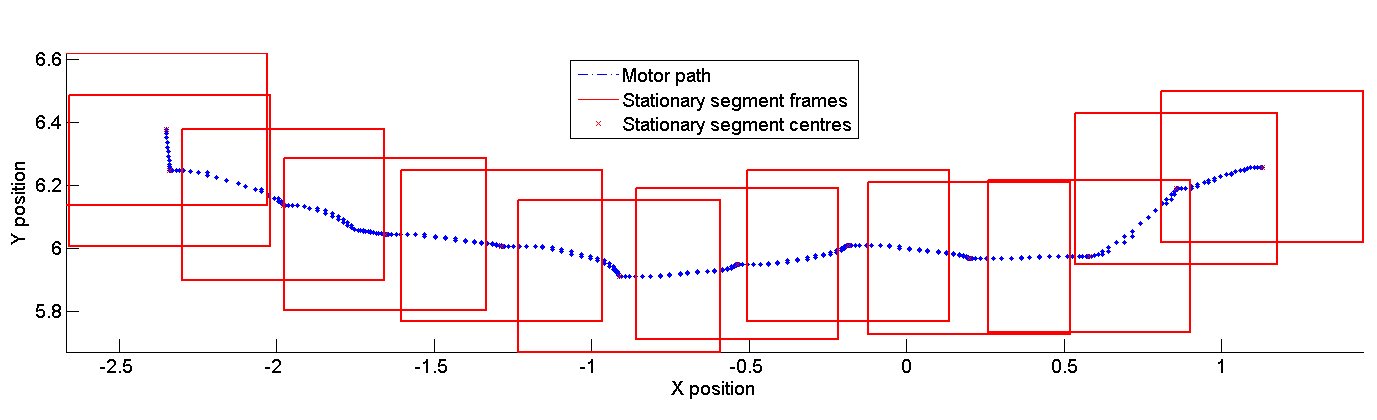
\includegraphics[width=0.98\columnwidth]{\figpath/sequence_trace_m.png}\\
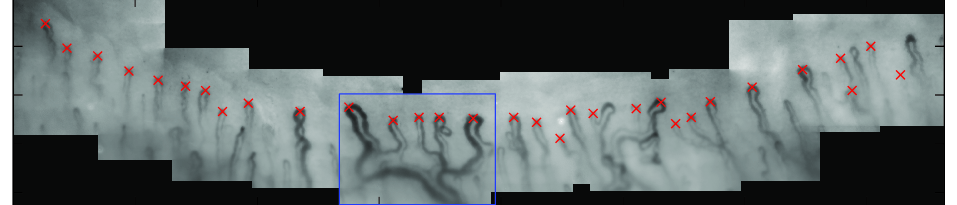
\includegraphics[width=0.98\columnwidth]{\figpath/pick_a_frame.png}\\
\noalign{\smallskip}
\end{tabular}
%
\caption{Generating mosaics; \textit{top}: video sequence motor positions are used to compute stationary segments and estimate the mosaic's global geometry; \textit{bottom}: a registered mosaic, with the distal capillaries detected. The blue box marks a stationary segment from which capillary videos }
\label{f:capillaroscopy}
\end{figure}
%
A complete video sequence of a nailfold typically comprises 10,000--20,000 raw frames, which are processed offline to generate high-quality static image mosaics and video sequences of each visible capillary. Consecutive frames can be separated into 3 types of segments where: 1) the motors are moving in the $(x,y)$-plane (\textit{panning}); 2) the z-motor is moving (\textit{focusing}); 3) the motors are stationary. The acquistion software limits continuous panning to guarantee stationary segments overlap, and only these frames are used to analyse capillaries (\fref{f:capillaroscopy}a). 
%However before discarding the non-stationary frames, we take their average to form an image in which everything except objects that remained stationary with respect to the camera (\eg~dust on the lens or sensor) are blurred out. The resulting dirt image is then subtracted from all stationary frames prior to further processing

First, frames within each segment are aligned and saved for later use in capillary videos (\sref{s:flow}). The aligned frames are averaged to form a compound frame with significantly lower noise and better contrast than the raw frames. The compound frames are then sequentially registered to form a mosaic image of the whole nailfold, using motor position as an initial alignment (\fref{f:capillaroscopy}). To guard against mis-registering frames with very little or no image content (a problem inherent in some nailfolds, both due to low-contrast and because disease may have destroyed capillary structure), frames that do not meet a minimum matching threshold are kept in their initial position, preventing total registration failure observed in earlier NC systems that employed mosaicking. This is particularly important where capillaries are only present/visible in some regions of a nailfold, as by keeping the global geometry of the mosaic intact, we can still safely measure capillary density.
%
\section{Measuring capillary structure}
\label{s:structure}
%
Having generated an image mosaic of the whole nailfold we use the method described by Berks et al.~\cite{Berks_MICCAI14} to detect the distal row of capillaries (\fref{f:capillaroscopy}b). The method first predicts pixel level estimates of vesselness ($V_s$~\ie~the probability of belonging to a vessel), vessel orientation ($V_\theta$) and width ($V_w$), as outputs from random forests trained on manually labelled capillaries, with features based on a multi-scale, multi-orientation decomposition of local image strcuture. The pixel level maps are used to apply a second level of machine learning in which scaled and rotated image patches are extracted from candidate vessel centres and used to predict the location of nearby capillary apices. A final selection of distal row capillaries can then be made using both local image appearance and the spatial relationships between the candidate apices.

As in~\cite{Berks_MICCAI14} we use the location of each distal capillary apex to compute capillary density (defined as the distance between the leftmost and rightmost distal capillaries, divided by the number of distal capillaries). In addition, using $V_s$ we compute the set of vessel pixels connected to, and at most 100$\mu$m from the apex of each capillary, and subsequently use $V_w$ and $V_\theta$ to compute the mean width $\mean{W}$ and orientation $\mean{\Theta}$ of each capillary. $\mean{W}$ is as a more robust measure of indiviudal capillary width than a point estimate at the apex and is used to compute mean and maximum capillary widths over the whole nailfold. 

Meanwhile, $\mean{\Theta}$, is used  to compute two further measures of structure: shape and derangement. Pixel orientations in $V_\theta$ are represented as angle-doubled unit vectors in the complex plane, $V_\theta(p) = \exp{2i\phi}$. Thus for each capillary  we can write $\mean{\Theta}$ as a complex number $S\exp{2i\mean{\phi}}$ where the magnitude  $S\in[0,1]$ is a measure of circular dispersion that will be higher in normal vessels (with long straight limbs and a narrow hairpin apex) than abnormally shaped capillaries. Taking the mean of each individual capillary dispersion $S$ across the image gives a measure of shape uniformity for the whole nailfold. 

Returning to $\mean{\Theta}$, the angle $\mean{\phi}$ represents the principal direction of the capillary. Discarding $S$, and taking the average of the unit vectors  $\hat{\Theta} = \exp{2i\mean{\phi}}$ across the nailfold generates a new mean orientation, the dispersion parameter of which $\mean{D}$ provides a measure of the uniformity of capillary direction (derangement), again with range $[0,1]$ and likely to be higher in nailfolds with normal structure.

The final set of structural measurements for each nailfold comprise capillary density, mean and maximum width, shape and derangement, approximately corresponding to measures made in earlier (semi-)manual quantitative analysis~\cite{Murray_etal_AR09}.
%
\begin{figure}[t]
\centering
\begin{tabular}{@{}c c c@{}}
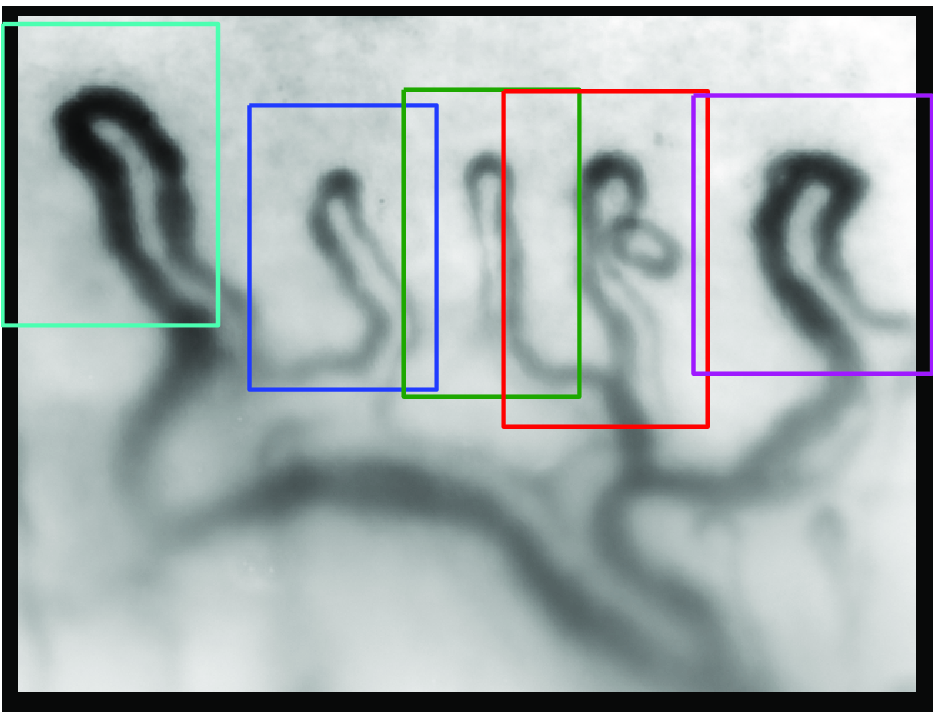
\includegraphics[width=0.52\columnwidth]{\figpath/segment_with_vessels.png} &
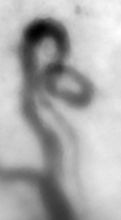
\includegraphics[width=0.22\columnwidth]{\figpath/vessel03.png} &
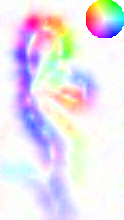
\includegraphics[width=0.22\columnwidth]{\figpath/vessel_fm03.png} \\
(a) & (b) & (c)\\
\noalign{\smallskip}
\end{tabular}
%
\caption{Measuring capillary flow: %
(a) capillary bounding boxes in a stationary segment; %
(b) average of re-registered cropped frames from the red box ready (see supplmentary material for video); %
(c) Estimate of vessel flow--colour denotes flow direction, intensity flow magnitude. %
}
\label{f:vessel_flow}
\end{figure}
%
\section{Measuring capillary flow}
\label{s:flow}
%
To build videos of capillary blood flow, we use the location of detected capillaries and the regsitered position of each compound frame in the nailfold mosaic to select the distal row capillaries visible in each stationary segment (\fref{f:vessel_flow}a). For a given segment, we use $V_s$ to define a bounding box around the extremeties of each capillary, and use this to sample patches from the segment's frames. 

The sampled patches for each capillary are re-registered using the compound frame, cropped to the capillary's bounding box, as a common target. This corrects pixel-level mis-registrations in the global frame alignment that make little difference when averaged in the static image, but significantly degrade flow estimation. Finally the registered patches are contrast normalised ready for flow estimation (\fref{f:vessel_flow}b).

To estimate blood velocity in a capillary video, we use a multiscale version of optical flow, based on the work of Brox et al.~\cite{BroxECCV04}. First, we form a pyramid stack of the patches, successively smoothing and downsampling the patches at each pyramid level. We then use least-squares non-linear optimisation to compute a dense flow field in the coarsest layer. This flow field is upsampled and used to warp the patches at the next pyramid level, before recomputing spatio-temporal gradients, and optimising again to find the new flow field. The process repeats until we reach the original image resolution.

The non-linear least-squares optimisation at each level combines a data term (that the pixels should obey the standard optical flow equations and thus maintain constant brightness~\cite{Horn_Schunk_AI81}) coupled with a smoothness term that acts to spatialy regularise the flow field (that nearby locations should have similar flow) while permitting non-linearities at object boundaries. We assume that flow is constant over time at any given location for the duration of the video, computing a single flow vector that optimally describes the observed horizontal and vertical displacements. At the finest pyramid level this effectively computes the mean flow over time at each pixel (\fref{f:vessel_flow}c). Measuring flow in this way is considerably more robust to noise than estimating flow between single pairs of frames, and is necessary to cope with the high-noise, low-contrast conditions inherent in NC imaging. 

To obtain a single measure of blood cell velocity for each capillary, we must account for the fact that a capillary may appear in multiple segments, or, particularly in the case of abnormally large capillaries, be split between segments. Rather than simply averaging flow measurements between segments, we project them back into the global geometry of the whole nailfold, and where they overlap, evaluate which segment produced a more reliable estimation. 

One option is to use the residual model fit from the top-level optimisation, although in practice we found this unreliable. Instead, we note that we do not constrain flow using $V_s$ or $V_\theta$ (although this is an interesting possibility for further work) and so the method will estimate non-zero flow outside of the vessel, and within the vessel may predict flow directions that do not match the predicted orientation. This provides two measures of flow reliability: firstly, using $V_s$ we compute the ratio of mean flow magnitudes inside and outside the vessel; secondly, using $V_\theta$ we measure the mean angular difference between the flow direction and orientation at each vessel pixel (doubling the angle of the flow vectors to make them invariant to direction).

In practice we found that selecting the segment which produced the highest vessel to background flow ratio gave best results, although work to validate measures of flow reliability are ongoing. Having projected estimations of flow from the capillary videos back to the global nailfold geometry, we take the mean flow magnitude over all distal capillaries as a single measure of blood velocity. %We note there are many other measures of flow we could consider (\eg~analysing the variations in flow, either spatially across the nailfold or temporally within each capillary), but as we show in~\sref{s:results}, preliminary results suggest mean flow velocity contains useful information, and given the capabilities of the new camera system we hope this is just the tip of the ice-berg in terms of investigating capillary blood flow using NC imaging.
%
\section{Experiments}
\label{s:experiments}
%
\subsection{Data}
\label{s:data}
112 subjects (50 HC, 12 PRP, 50 SSc) were recruited in a tertiary referral centre for SSc and imaged using the new system. Video sequences of all 10 digits (where available) were acquired, generating 1,104 sequences.  A total of 23,489 distal capillaries were detected and used to compute measures of capillary density, mean and maximum width, shape, derangement and mean flow velocity. For each subject we computed the mean over all their gradeable digits to produce a single value for each parameter (8 subjects had one or more ungradeable digits, although all had at least 3 gradeable digits).
%
\subsection{Results}
\label{s:results}
%
\begin{figure}[t]
\centering
\begin{tabular}{@{}c c@{}}
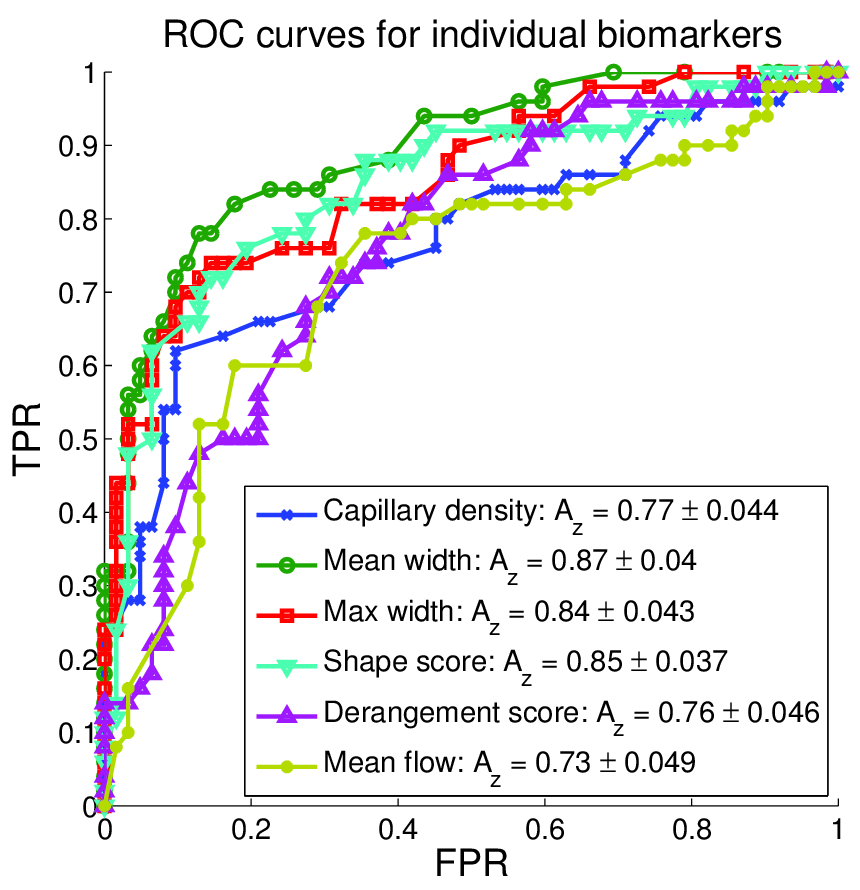
\includegraphics[width=0.48\columnwidth]{\figpath/individual_rocs.png} &
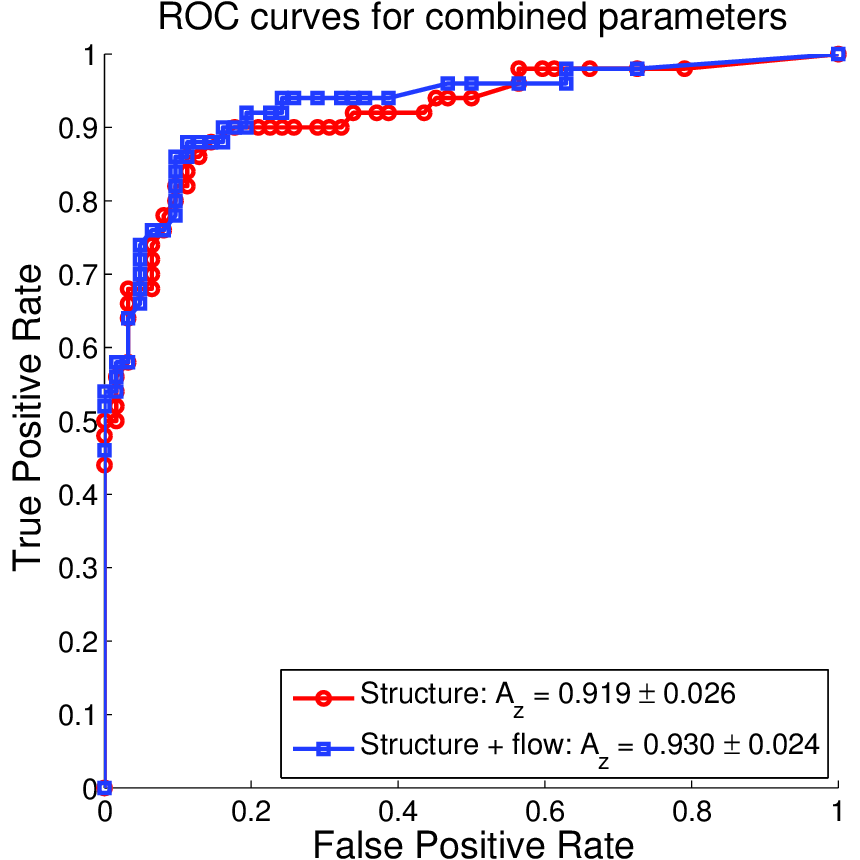
\includegraphics[width=0.48\columnwidth]{\figpath/combined_rocs.png} \\
(a) & (b)\\
\noalign{\smallskip}
\end{tabular}
%
\caption{ROCs for separating HC and PRP from SSc: %
(a) Indiviudal measures of capillary structure and flow; %
(b) combined measures in a logistic regression model, with and without flow.
}
\label{f:subject_rocs}
\end{figure}
%
\begin{table}[tb]
\centering
%\small
\input{results_table.txt}
%
\caption{Group means and standard errors and ROC $A_z$ values for each capillary measure. $\sharp$, $\dagger$, $\ddagger$ denote significant pair-wise differences for PR vs HC, SSc vs HC, and SSc vs PR respectively.}
\label{t:results}
\end{table}
%
Group means and standard errors for each structure and flow parameter are shown in \tref{t:results}. The group means for SSc are statistically significantly different to both HC and PRP for all parameters, with values that match results from earlier trials (including both manual and automated analysis)~\cite{Murray_etal_AR09,Berks_MICCAI14}. For each individual parameter ~\fref{f:subject_rocs}a shows an ROC curve and $A_z$ values for predicting SSc (positive) versus the combined group HC/PRP (negative).

We combined the individual parameters in a logistic regression model using  HC/PRP vs SSc as a binary output variable, first using only the structural measures and then including flow. Stepwise regression was used to add/remove terms from an initial linear model fit, and in both cases max width (highly correlated with mean width) and derangement (highly correlated with shape) were discarded. In the latter model flow was retained suggesting it provides additional independent information to the structural measures. To estimate model performance we applied leave-one-out cross-validation to obtain unbiased predictions for each subject (\fref{f:subject_rocs}b). The model of structural measures produced an $A_z$ of 0.919, significantly greater than the best single parameter (mean width $A_z$ = 0.874). Including flow further imrpoved performance ($A_z$ = 0.930), again indicating that flow contains complementary information for diagnosing SSc.
%
\section{Conclusions}
\label{s:conclusions}
We have presented details of a new nailfold capillaroscopy system that we believe enhances the current state-of-the-art of in-vivo microvascular imaging. Carefully selected hardware components, combined with novel, bespoke software, enables fast and easy acquisition of high-quality video sequences in which both capillary structure and blood velocity are measured automatically. We have shown the results of an initial trial of the system in a case/control study in which capillary measures strongly predict patients with SSc. Blood flow velocity results, while preliminary, are promising and warrant further investigation, and we are currently working on validating the results, including psychovisual tests with human observers and  developing a microscopic flow phantom to provide objective ground truth.

To test the sensitivity of flow measures, we are planning trials that include dynamic challenges to induce rapid changes in capillary function. Moreover the optical properties of the system may easily be adapted to assess other measures of capillary function (\eg~using multispectral imaging to assess oxygenation, or UV induced fluorescence  to measure oxidative stress), providing an exciting avenue for further investigations of pathophysiology and microangiopathy. 

%\textbf{Acknowledgements.}
%This work was funded by the Wellcome Trust. We are grateful to all the observers that annotated images used in the study.
%\end{document}

\bibliographystyle{splncs}
\bibliography{./bib/_aliases,./bib/miccai2016}

\end{document}
